

\documentclass[a4paper,11pt]{article}
\usepackage[french]{babel}% Package Babel pour le texte en francais
\usepackage{exptech}% Presentation similaire a celle de l'expose technique
\usepackage{graphicx} % Pour les images
\usepackage{url}

% Titre
\title{\textbf{Surveillance environnementale intelligente pour le campus}}

% Auteurs
\author{DUBOIS Mathys,	ZAKY Marc,	LE PELVE Maxime,	NUSS Iwen,\\	DUBUC--TABOUY Amaury
	\\ \\
	Encadrant : NIKOLAOS PARLAVANTZAS}

\date{2024-2025}                    % Ne pas modifier

\begin{document}

	
	\maketitle
	\section*{Résumé}
	Le changement climatique accéléré et les activités humaines imposent un suivi plus précis de la faune et de l'environnement. Ce projet vise à développer un système de suivi intelligent capable de détecter automatiquement la présence d'animaux à l'aide d'une caméra. Dans cette étude, nous avons conçu une solution embarquée reposant sur un Raspberry Pi 3 et une caméra Pi, capable de capturer des images sur le terrain. Le traitement des données est effectué localement (Fog Computing) pour minimiser la latence avant d'être envoyé à une plateforme serverless.
	
	%\tableofcontents
	
	\section{Remerciements}
	Nous souhaitons adresser nos sincères remerciements à notre encadrant, M. Nikolaos Parlavantzas, pour son accompagnement, son engagement constant et la qualité de ses conseils tout au long de l’année.
	
	\section{Introduction}
	Dans un contexte de bouleversements climatiques accélérés, le besoin de suivre en temps réel l’évolution de la faune et de l’environnement devient essentiel. En parallèle, les avancées technologiques en matière de capteurs connectés, d'intelligence artificielle et de traitement distribué offrent de nouvelles perspectives pour observer la nature de manière fine et automatisée.\\
	Dans ce contexte, nous avons développé un système de suivi environnemental intelligent, capable de détecter automatiquement la présence d’animaux à l’aide d’une caméra embarquée. Ce projet s’inscrit au sein de l'étude pratique des 4INFO nommé Mycelium qui vise a étudier la renaturalisation de la Croix Verte, un espace vert situé à proximité de la station Beaulieu-Université sur la ligne B du métro de Rennes. Cette zone, récemment impactée par des aménagements urbains, constitue un terrain d’observation privilégié pour évaluer les effets de la renaturation sur la biodiversité locale.

	\section{Cahier des charges}
	\subsection{Objectifs}
	L’objectif de cette étude pratique est de développer une application d’analyse vidéo basée sur l’intelligence artificielle et de l’intégrer au sein du système Mycélium. Cette application devra traiter un flux vidéo en temps réel, analyser son contenu à l’aide d’algorithmes d’IA, stocker des données historiques et générer des alertes en fonction des éléments détectés. Elle sera conçue sous la forme d’un ensemble de fonctions FaaS réparties entre les objets connectés, la couche fog et le cloud. Le développement s’appuiera sur un prototype initial réalisé par un groupe d’étudiants de l’INSA, qui permettait de recenser les animaux présents sur le campus. Ce prototype reposait sur un Raspberry Pi équipé d’une caméra et sur un serveur exécutant un modèle de classification d’images pré-entraîné.
	\subsection{Fonctionnalités attendues}
	\begin{enumerate}
	\item Détection de mouvement via flux vidéo localisé sur Raspberry Pi.
	\item Analyse d’images pour identifier les animaux détectés.
	\item Tri et filtrage des données pour éviter les doublons ou mauvaises détections.
	\item Transfert des données vers le serveur distant.
	\item Traitement et reclassement des données avec un modèle amélioré.
	\item Stockage des données dans une base de données interrogeable.
	\item Système d’alerte (notifications Discord lors de la mise à jour de la base).
	\item Intégration dans le cluster Mycélium.
	\end{enumerate}
	
	\section{État de l'art}
	Dans le cadre de ce projet, plusieurs initiatives existantes ont été étudiées afin de comprendre les approches actuelles en matière de suivi automatisé de la biodiversité par l'intelligence artificielle.
	
	\subsection{DeepFaune}
	DeepFaune est un projet français initié en 2022 par des chercheurs du CNRS (Institut National d’Écologie et d’Environnement - INEE). Il s’appuie sur des pièges photographiques équipés de capteurs de mouvement pour capturer automatiquement des images d’animaux dans leur habitat naturel. Ces images sont ensuite traitées par des algorithmes d’intelligence artificielle permettant une identification rapide et fiable des espèces. Cette technologie vise à faciliter et à accélérer le travail des chercheurs en réduisant considérablement le temps consacré à l’analyse manuelle. Toutefois, elle nécessite encore une récupération physique régulière des données sur les pièges photographiques, ce qui peut représenter une contrainte sur le terrain. \cite{deep}
	\subsection{Wildlife Insights}
	Wildlife Insights est une plateforme internationale collaborative lancée en 2019 avec le soutien d'organisations majeures telles que Google et le WWF. Son objectif est de centraliser et d’analyser des millions de photos capturées par des pièges photographiques à travers le monde, en s’appuyant sur des algorithmes avancés de reconnaissance d’images. Cette initiative facilite les comparaisons interrégionales et appuie les politiques de conservation en offrant une base de données mondiale sur la biodiversité accessible à l’ensemble de la communauté scientifique et environnementale. Toutefois, le système ne permet pas la récupération des données à distance, ce qui impose une collecte manuelle sur le terrain.\cite{wild}
	\subsection{Mycélium}
	Mycélium est un projet lancé en 2022 par des étudiants de l’INSA Rennes, en partenariat avec le laboratoire Géosciences Rennes, dans le cadre du programme TERRA FORMA du CNRS. Il avait pour objectif d’étudier la renaturalisation de la Croix Verte, un espace récemment affecté par des aménagements urbains. Le projet se divisait en deux volets : le premier portait sur l’analyse des évolutions climatiques grâce à des capteurs environnementaux, tandis que le second visait à détecter en temps réel la présence d’un renard à l’aide d’une caméra. Notre projet s’inscrit dans la continuité de Mycélium 2.0, avec pour ambition de l'améliorer significativement en élargissant la détection à un plus grand nombre d'animaux et en optimisant le traitement en local grâce au fog computing.\cite{mycelium}

	\section{Architecture}
	\subsection{Outils}
	Pour répondre à nos objectifs et à l’architecture choisie, nous avons utilisé divers outils :
	\begin{enumerate}
			
	\item \textbf{Raspberry Pi 3B et Raspberry Pi Caméra Module 2 :} Le système repose sur un Raspberry Pi modèle 3B, couplé au Raspberry Pi Camera Module 2, permettant de capturer des images en haute définition. Le Raspberry Pi est un nano-ordinateur compact, peu coûteux, largement utilisé pour des projets embarqués et éducatifs. Ce matériel est idéal pour le traitement local des données et l’analyse des vidéos, tout en étant facilement déployable.
	
	\item \textbf{Faasd :} Le modèle FaaS (Function-as-a-Service) permet d’exécuter des fonctions de manière serverless, c’est-à-dire sans avoir à gérer l’infrastructure sous-jacente, avec des avantages tels que la scalabilité, l’isolation des fonctions et une grande simplicité de déploiement. OpenFaaS est une solution open source qui met en œuvre ce modèle. Sur le Raspberry Pi, nous avons utilisé faasd, une version légère et simplifiée d’OpenFaaS, ne nécessitant pas de cluster Kubernetes et fonctionnant sur un seul hôte. Cela le rend idéal pour les environnements contraints, car il permet d’exécuter des fonctions serverless localement avec un minimum de ressources. \cite{faasd}
	
	%\item \textbf{OpenFaaS :} Sur le serveur distant, nous avons déployé OpenFaaS, une plateforme complète de fonctions serverless. Elle permet d’héberger et d’exécuter les fonctions de traitement plus lourdes, comme le tri des images ou l’analyse statistique, dans un environnement plus puissant et évolutif. Grâce à son API RESTful et sa compatibilité Docker, OpenFaaS facilite le déploiement, la montée en charge et la maintenance des fonctions.
	
	\item \textbf{SQLite :} Le système de gestion de base de données SQLite a été choisi pour sa simplicité et son efficacité. Contrairement à InfluxDB, qui est orienté vers les séries temporelles, SQLite offre une solution légère, idéale pour un projet localisé et embarqué. Il permet de gérer les données relatives aux animaux détectés, aux photos et aux événements de manière optimale, tout en étant facile à utiliser avec Python grâce à des bibliothèques dédiées.\cite{sqlite}
	
	\item \textbf{YOLO :} Pour l’analyse des images, nous avons intégré YOLO (You Only Look Once), un modèle de détection d’objets en temps réel. YOLO permet de classifier et localiser les animaux présents dans les images capturées par le système de caméras, offrant ainsi une détection rapide et précise. \cite{yolo}
	
	\item \textbf{NATS :} NATS est un système de messagerie léger et performant permettant la communication asynchrone entre différents composants d'une application distribuée. Il permet d’envoyer des données sur des topics spécifiques, que les fonctions abonnées peuvent ensuite récupérer. Cela facilite grandement les échanges entre les différentes parties du système. \cite{docnats}
	
	\item \textbf{Docker :} Nous avons utilisé Docker pour l’hébergement des fonctions. Grâce à Docker, nous avons pu regrouper nos fonctions dans des containers qui peuvent être facilement déployés sur n’importe quelle infrastructure FaaS. Cela simplifie le déploiement sur des périphériques tiers et assure une gestion fluide des fonctions.
	
	\end{enumerate}	
	
	Enfin, tout ce travail se déroule dans le Fog Computing, qui agit comme un Cloud local. Le traitement est effectué sur place, à proximité des dispositifs de détection, et les résultats sont ensuite envoyés vers le Cloud, où les informations sont centralisées et mises à la disposition des utilisateurs et utilisatrices.

	\subsection{Structure}
		\begin{figure}[ht]
			\centering
			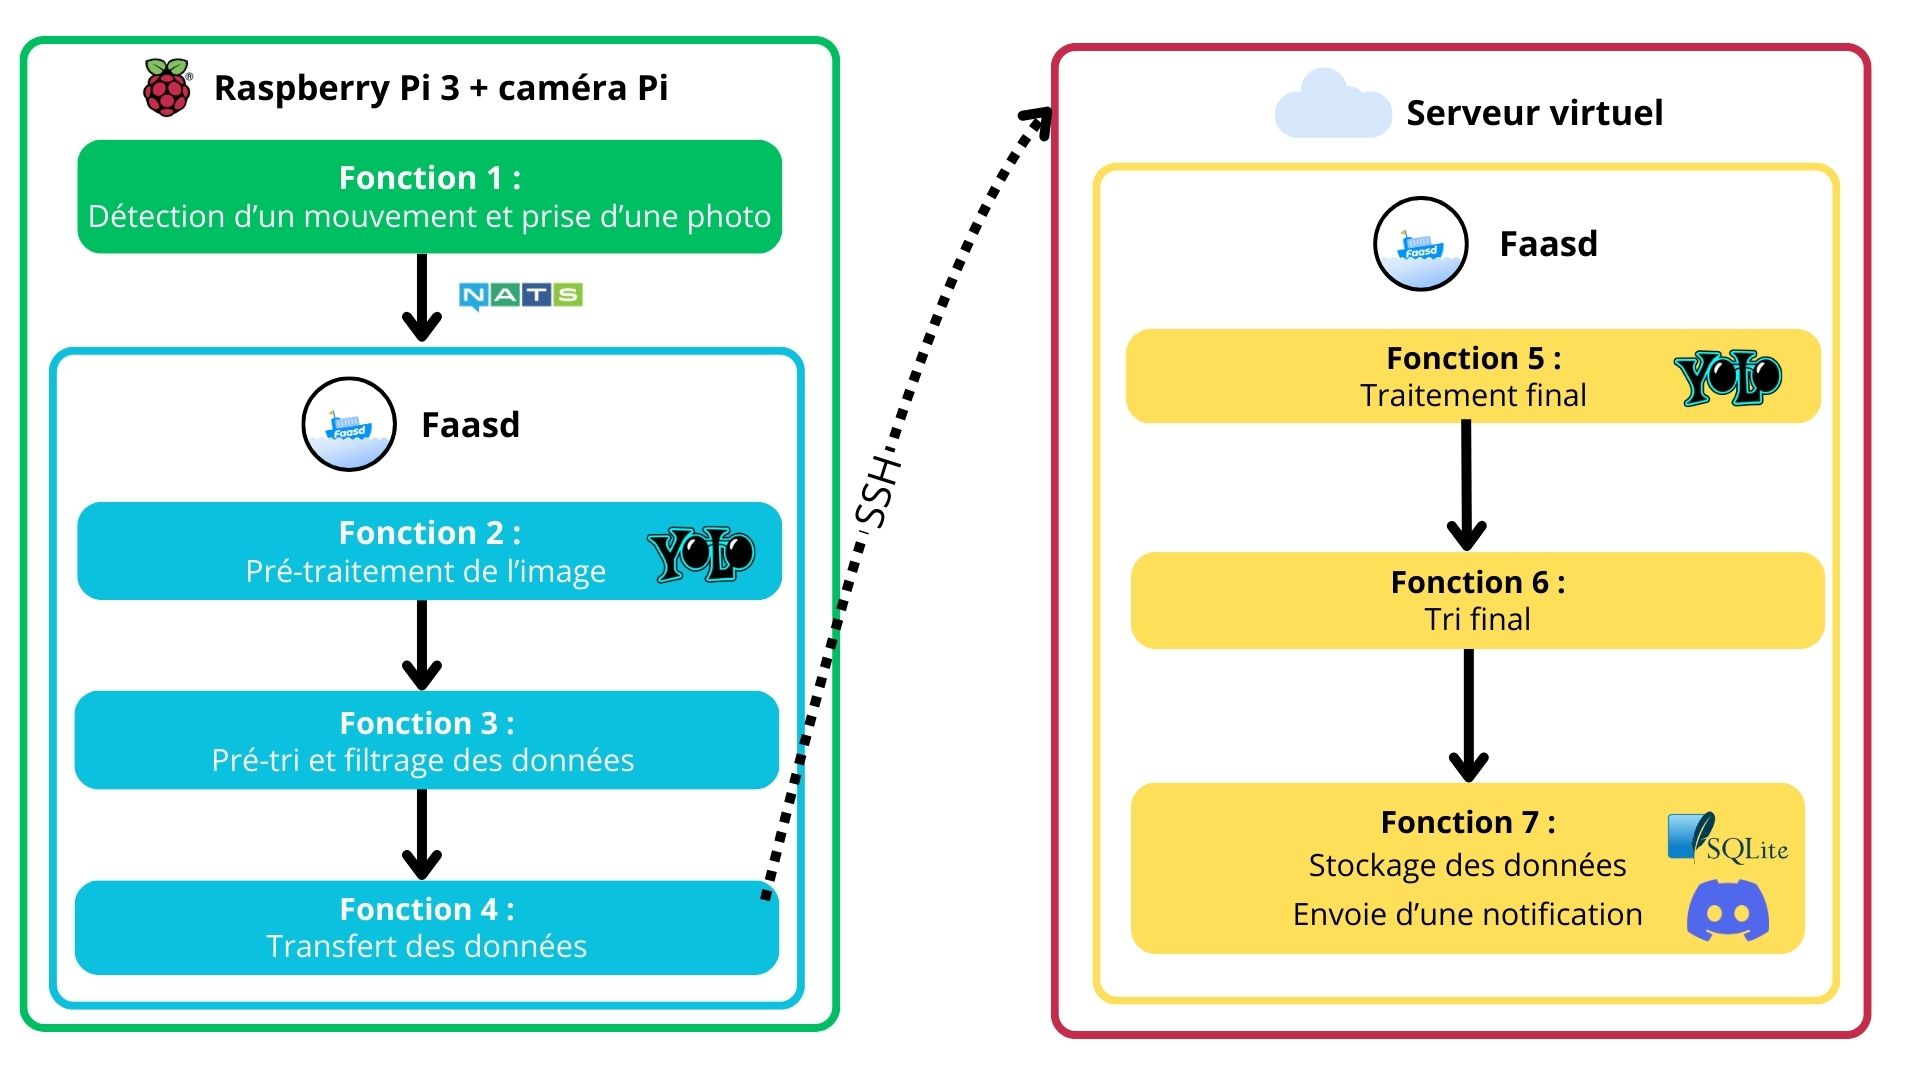
\includegraphics[scale=0.25]{architectureFinale.jpg}
			\caption{Architecture du projet}
			\label{fig1}
		\end{figure}
	L’architecture générale de notre système est illustrée dans la figure ci-dessus. Elle repose sur une séparation claire entre les traitements réalisés localement sur le Raspberry Pi et ceux déportés sur un serveur distant. Cette organisation vise à maximiser les traitements embarqués — notamment la détection de mouvements et l’identification des animaux via le modèle YOLO — afin de réduire au strict nécessaire les transferts de données, coûteux en énergie et en bande passante.
	
	L’ensemble des modules a été développé en Python, un langage que nous maîtrisons bien et qui offre un riche écosystème pour le traitement d’image, l’intelligence artificielle et la communication inter-processus. Les interactions entre les différents composants sont orchestrées via le protocole de communication NATS, léger et performant, qui facilite la transmission asynchrone des messages entre les modules locaux et le serveur distant.
	
	Ce découplage entre le traitement embarqué (capture, détection, filtrage) et le traitement distant (tri, stockage, analyse) permet une architecture flexible, économe en ressources et facilement évolutive.



	
	\section{Fonctionnalités réalisées}
	\begin{enumerate}
		
		\item \textbf{Détection de mouvement et capture d'image :}  
		Cette première fonction s'exécute en continu sur le Raspberry Pi et permet de détecter des mouvements devant la caméra. Elle compare les pixels de deux images successives (prises à l’instant $t$ et $t+1$) et déclenche une capture si la différence dépasse un certain seuil, traduisant un mouvement significatif. L’image capturée est alors enregistrée localement sur le Raspberry Pi. Pour éviter la prise de multiples photos d’un même animal en mouvement, un délai arbitraire de 10 secondes est appliqué avant une nouvelle détection.\\
		
		\item \textbf{Pré-traitement de l'image :}  
		Une seconde fonction utilise le modèle de détection YOLOv8 pour analyser l’image capturée. Les résultats de cette détection sont enregistrés dans un fichier Json contenant, pour chaque objet détecté : le nom de la classe prédite, le nombre d’occurrences, le niveau de confiance du modèle, la date et l’heure de la détection, ainsi que le chemin vers l’image.
		\begin{figure}[ht]
			\centering
			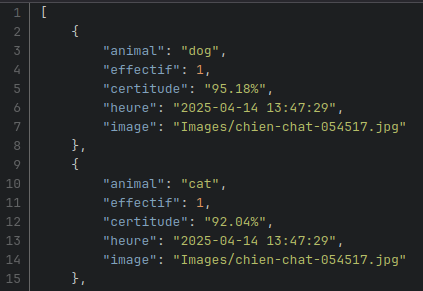
\includegraphics[scale=0.3]{json.png}
			\caption{Données des détections en format Json}
			\label{fig2}
		\end{figure}
		
		\item \textbf{Pré-tri et filtrage des données :}  
		Étant donné les limitations de ressources du Raspberry Pi, nous utilisons un modèle YOLOv8 non ré-entraîné, capable de détecter dix espèces animales courantes. Ce modèle peut également détecter d'autres objets non-animaux. Nous avons toutefois constaté qu’en présence d’un animal non reconnu, YOLOv8 propose malgré tout une prédiction parmi les classes animales connues.  
		La première tâche de cette fonction est donc de ne conserver que les détections interprétables comme animales, tout en excluant explicitement les détections de personnes humaines (afin de préserver la vie privée). La seconde tâche consiste à éliminer les doublons, en comparant la date de capture et les classes détectées : cela permet de ne pas conserver plusieurs images du même animal prises à quelques secondes d’intervalle.\\

		
		\item \textbf{Transfert des données :}  
		Cette fonction gère l’envoi des données collectées depuis le Raspberry Pi vers le serveur distant. Le fichier JSON contenant les informations de détection, ainsi que le dossier des images, sont d’abord transférés via SSH. Une fois le transfert effectué, le Raspberry Pi envoie un message via NATS pour déclencher le début du traitement sur le serveur. L’envoi peut être déclenché automatiquement à intervalles réguliers (toutes les 24 heures) ou dès qu’un seuil de 10 nouvelles images est atteint.\\
		
		\item \textbf{Traitement final :}  
		Sur le serveur, une nouvelle fonction utilise un modèle YOLO que nous avons ré-entraîné avec un jeu de données spécifique à la faune locale (notamment celle présente sur le site de la Croix Verte). Cette étape vise à affiner la classification et réduire les erreurs. Chaque image transmise est ré-analysée, et les nouvelles données de détection sont enregistrées dans un nouveau fichier Json.
		\begin{figure}[ht]
			\centering
			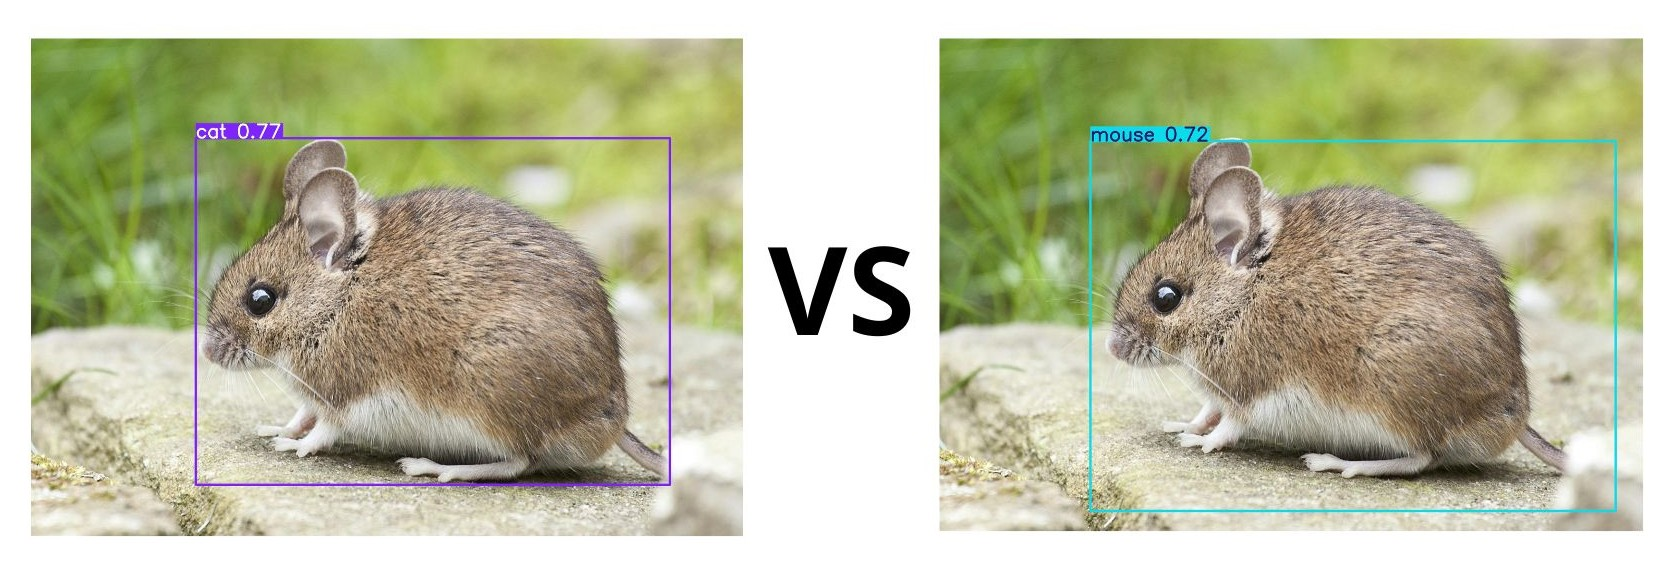
\includegraphics[scale=0.18]{souris.jpg}
			\caption{Pré-traitement (cat) vs traitement final (mousse)}
			\label{fig3}
		\end{figure}		
		\item \textbf{Tri final :}  
		Une deuxième étape de tri est ensuite appliquée. Elle vise à détecter et éliminer d’éventuels doublons restants, mis en évidence par la seconde classification. Comme pour le pré-tri, on compare la date de capture et les classes détectées pour regrouper ou supprimer les images redondantes d’un même animal ayant été interprété différemment.\\
		
		\item \textbf{Stockage des données et envoie d'une notification :}  
		Les données issues du fichier JSON final sont insérées dans une base de données SQLite. Afin de structurer au mieux l’information et de faciliter les requêtes ultérieures, nous avons choisi de répartir les données en deux tables : l’une contenant les informations relatives aux animaux détectés(photo, classe de l'animal, nombre d’animaux de la même classe), l’autre les métadonnées des photos (heure, date, nombre d’animaux). Cette organisation optimise l’interrogation via une interface de consultation dédiée. Une fois la base de données mise à jour, une notification est automatiquement envoyée via un serveur Discord afin d’informer les utilisateurs que de nouvelles données sont disponibles. Cette notification permet un suivi en temps réel de l’activité du système.
		\begin{figure}[ht]
			\centering
			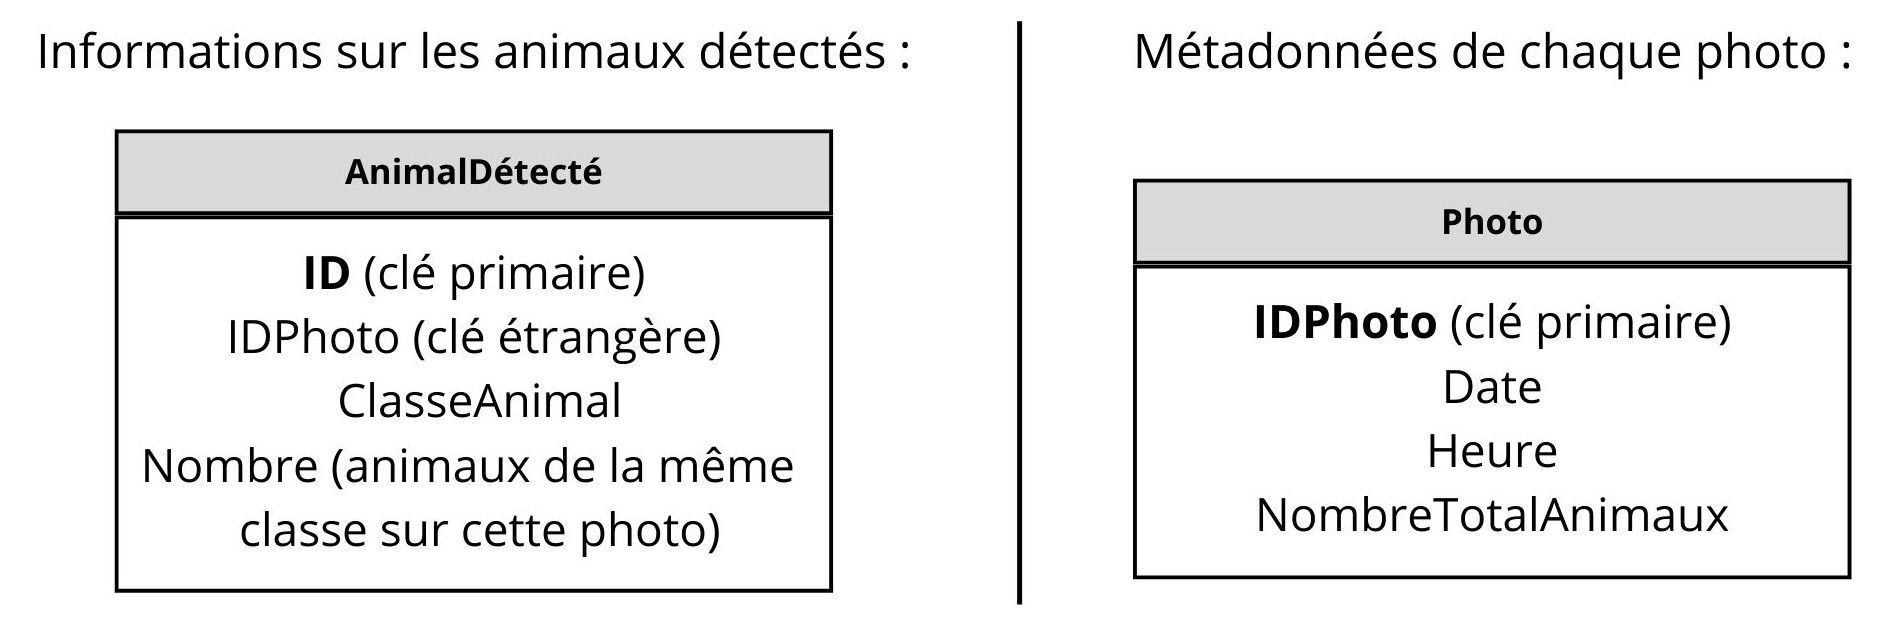
\includegraphics[scale=0.15]{BDD2.jpg}
			\caption{Tables de la base de données}
			\label{fig4}
			
		\end{figure}
		\vspace{0.4cm}
		\begin{figure}[ht]
			\centering
			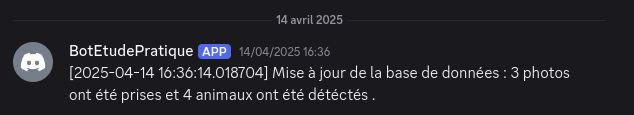
\includegraphics[scale=0.4]{Discord.png}
			\caption{Réception de la notification Discord}
			\label{fig5}
		\end{figure}
		
	\end{enumerate}
	
	\section{Résultats}
	Au terme de notre projet, nous avons pu valider l’ensemble des fonctionnalités définies dans notre cahier des charges. Le système développé fonctionne de manière autonome et fiable, avec une séparation claire et efficace entre les traitements réalisés localement sur le Raspberry Pi et ceux déportés sur le serveur distant.
	
	L’architecture que nous avons conçue présente l’avantage d’être modulaire et facilement évolutive. Il est ainsi possible d’adapter le système à d’autres contextes ou types d’animaux en ré-entraînant simplement le modèle YOLO utilisé dans la phase de traitement final. Par exemple, en entraînant un modèle spécifique aux espèces d’oiseaux, il devient possible de cibler plus précisément la faune souhaitée sans modifier l’architecture générale du projet.
	
	Globalement, notre système a permis de détecter et classifier plusieurs espèces animales, tout en utilisant des ressources limités. Les tests réalisés ont confirmé la viabilité de notre approche, tant sur le plan technique que fonctionnel.


	\section{Difficultés rencontrées}
	Au cours de la réalisation de notre projet nous avons été confrontés à plusieurs difficultés techniques et organisationnelles.\\
	
	L'une des principales difficultés techniques a été la limitation en mémoire vive (RAM) du Raspberry Pi 3, qui ne permettait pas d'utiliser les outils initialement prévus pour la mise en œuvre de notre architecture serverless, notamment OpenFaaS et Kubernetes, tous deux trop gourmands en ressources. Nous avons donc dû nous orienter vers des solutions plus légères, comme FaaSd, mieux adaptées aux contraintes de l’embarqué. Cependant, l’utilisation de FaaSd a soulevé d'autres problèmes : la documentation technique est quasi inexistante et les ressources en ligne sont très limitées. Le manque de ressources a nécessité une optimisation poussée du code, ainsi qu’un arbitrage entre ce qui pouvait être traité en périphérie (Fog computing) et ce qui devait être déporté vers le cloud (FaaS).\\
	
	De plus, la caméra Pi utilisée dans notre prototype s’est révélée de faible qualité, avec une résolution limitée et un temps de latence élevé entre chaque prise de vue. Ce qui affecte la précision et la réactivité de notre système de détection.\\
	
	Concernant l'organisation du travail, nous avons également rencontré des difficultés pour collaborer à distance sur le Raspberry Pi. Bien que nous ayons mis en place une solution permettant de prendre le contrôle de la machine à distance, cette dernière ne supportait que quatre connexions simultanées, ce qui excluait systématiquement un membre de notre groupe de cinq.\\
	
	Nous avons également rencontré des difficultés lors de l'entraînement de notre propre modèle YOLO, dans le but de l’améliorer en le fusionnant avec le modèle préexistant. Malheureusement, cette opération s’est révélée impossible . Nous avons donc dû entraîner un modèle complet, en collectant et en annotant des images pour plusieurs espèces animales. Ce processus, particulièrement chronophage, a nécessité des efforts importants pour constituer un jeu de données représentatif et atteindre un niveau de précision acceptable.\\
	
	Par ailleurs, l’intégration du modèle de détection YOLO (You Only Look Once) s’est heurtée à une incompatibilité avec FaaSd, la solution Function-as-a-Service que nous avions adoptée par contrainte matérielle. FaaSd ne prend pas en charge la version récente de YOLO que nous utilisions, ce qui a limité nos possibilités d’exploitation du modèle directement dans l’architecture serverless.
	

	\section{Conclusion}
	Ce projet nous a permis de concevoir, développer et tester une solution embarquée de détection d’animaux intégrant des technologies modernes telles que YOLO, OpenFaaS/faasd, NATS et SQLite. L’objectif initial – surveiller une zone naturelle de manière automatisée tout en limitant les ressources utilisées – a été atteint. Faute de temps et en raison de contraintes d’emploi du temps, nous n’avons malheureusement pas pu intégrer notre solution au projet Mycélium. Toutefois, cette intégration n’aurait pas posé de difficulté majeure : il suffirait de transférer les fonctions sur le serveur de Mycélium et de configurer le réseau. L’essentiel du travail, à savoir le développement, a déjà été réalisé.
	
	Nous avons démontré qu’il était possible de combiner des traitements locaux légers (sur Raspberry Pi) avec des traitements plus poussés côté serveur, grâce à une architecture modulaire et découplée. Le recours aux fonctions serverless a permis d’assurer la maintenabilité, la modularité et la simplicité de déploiement du système.
	
	L’ensemble du système est aujourd’hui fonctionnel, et son architecture permet de l’étendre à d’autres zones de surveillance ou d’autres types d’analyses (par exemple : détection de comportements, suivi temporel des espèces, analyse statistique de fréquentation). Des pistes d’amélioration peuvent être envisagées, notamment :
	
	\begin{itemize}
		\item L'amélioration de la caméra pour avoir des images de meilleures qualités et utiliser une caméra infrarouge pour pouvoir faire des détections nocturnes.
		\item L'optimisation du modèle de détection afin d'être plus précis et de détecter une plus grande diversité d'animaux.
		\item Le développement d’une interface web plus avancée pour la visualisation des données et des statistiques.\\
	\end{itemize}
	
	En somme, ce projet nous a offert une expérience riche mêlant traitement d’image, intelligence artificielle, développement embarqué, communication distribuée et gestion de base de données. Il ouvre la voie à des applications concrètes dans le domaine de la surveillance environnementale intelligente.
	
	\bibliography{BiblioEP}
	

\end{document}


